\documentclass[a4paper,11pt]{article}
%\usepackage[utf8]{inputenc} % utf8 c'est la norme
\usepackage[applemac]{inputenc}

\usepackage[frenchb]{babel}
\usepackage{graphicx}
\usepackage{float}

\usepackage[top=2.5cm, bottom=2.5cm, left=2.5cm, right=2.5cm]{geometry}

\usepackage[pdfauthor={Agathe Oddon, Jean-Michel Tozzini},%
pdftitle={IC03 - Rapport de cours},%
pagebackref=true,%
pdftex,%
linkcolor=blue,%
colorlinks]{hyperref}

\begin{document}
\title{LO21 : Rapport de projet\\Calculatrice � notation polonaise invers�e}
\author{Agathe Oddon\\Jean-Michel Tozzini}
\date{Printemps 2012}

\maketitle

\section*{Introduction}
Dans le cadre de notre UV LO21, nous devions r�aliser la conception puis impl�menter en C++ une calculatrice � notation polonaire invers�e.

Le rendu final du projet est compos� du pr�sent rapport, du code du programme ainsi que de  sa documentation Doxygen.

\tableofcontents

\section{Conception}
\subsection{Diagramme de classes}
\begin{figure}[H]
	\center
	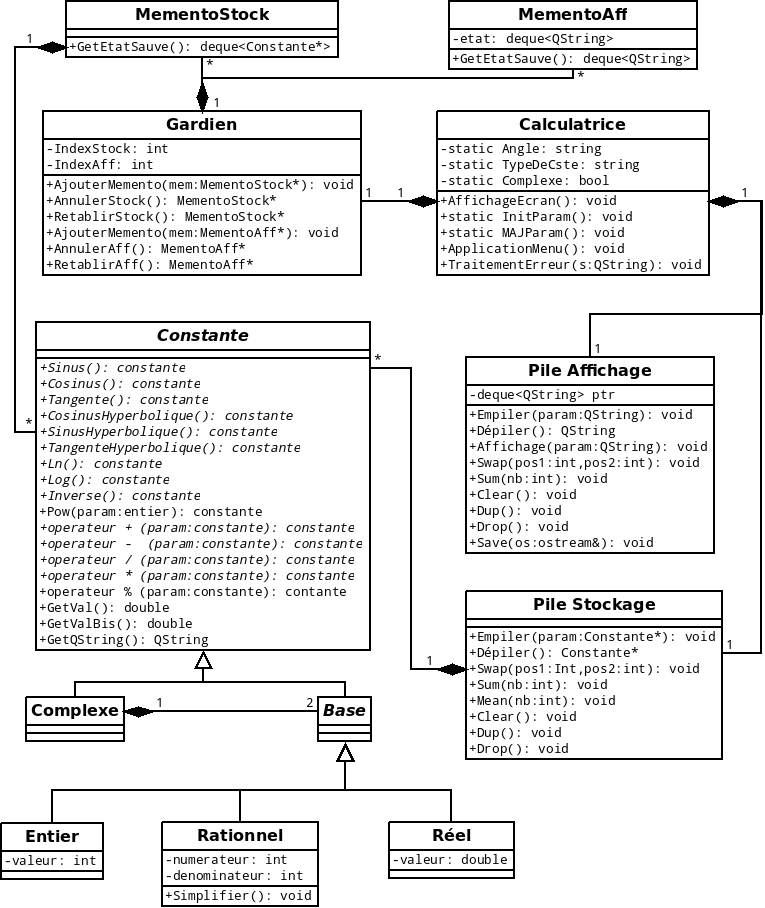
\includegraphics[width=16.7cm]{UMLProjetLO21v3.png}
	\caption{Diagramme de classe de la Calculatrice � notation polonaise invers�e}
\end{figure}
\subsubsection{Types de donn�es}
Nous avons choisi de repr�senter les donn�es manipul�es par la calculatrice comme des objets de trois classes : Entier, R�el, Rationnel, Complexe et Expression. 

La classe complexe est compos�e de deux objets de type Base, classe abstraite de laquelle d�rivent Entier, R�el et Rationnel. Cela permet d'obtenir des complexes compos�s de deux attributs de types diff�rents.

Les classes Base, Complexe et Expression d�rivent de la classe abstraite et exclusive Constante. 

L'utilisation de la classe m�re abstraite Constante nous permet � la fois d'empiler des objets de type pointeur sur Constante, et de d�finir des m�thodes polymorphes pour les op�rateurs. 

- Pourquoi deux piles ?

- Renvoi type le plus riche, sauf Rationnel\&Reel



\subsection{Diagrammes de s�quences}
\begin{figure}[H]
	\center
	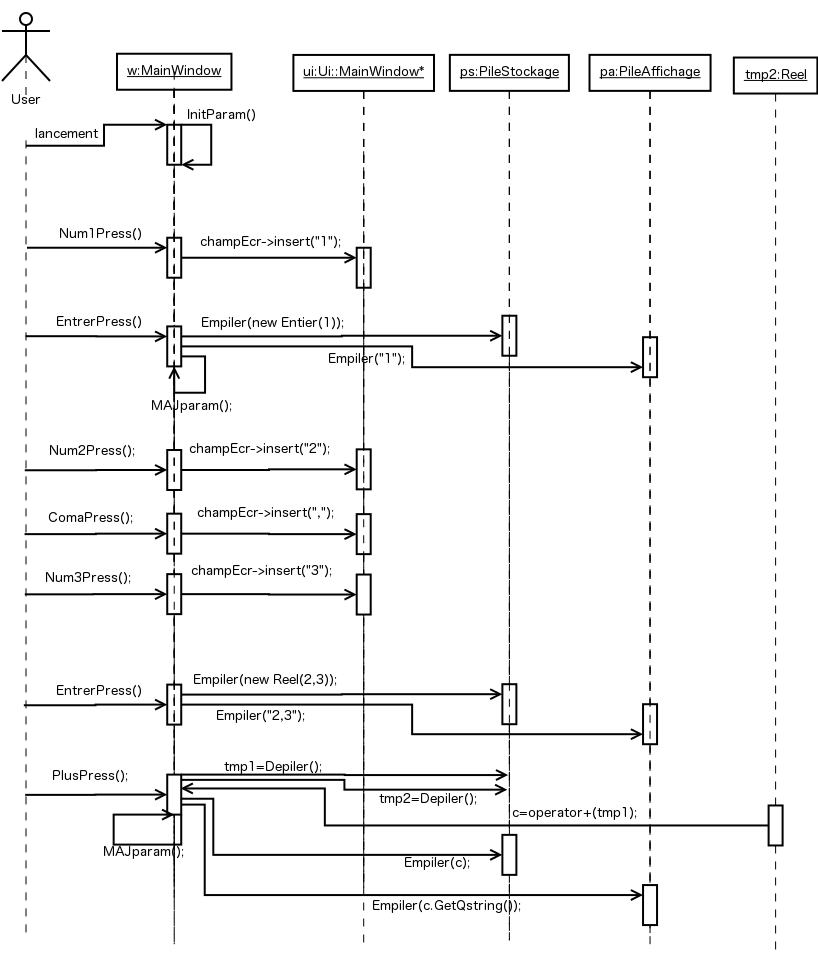
\includegraphics[width=16.7cm]{diag_seq_1.png}
	\caption{Diagramme de s�quence d�crivant le lancement de la fen�tre, la saisie de "1", "2,3" , l'appui sur le bouton "+" par l'utilisateur, puis l'addition des deux valeurs.}
\end{figure}

\begin{figure}[H]
	\center
	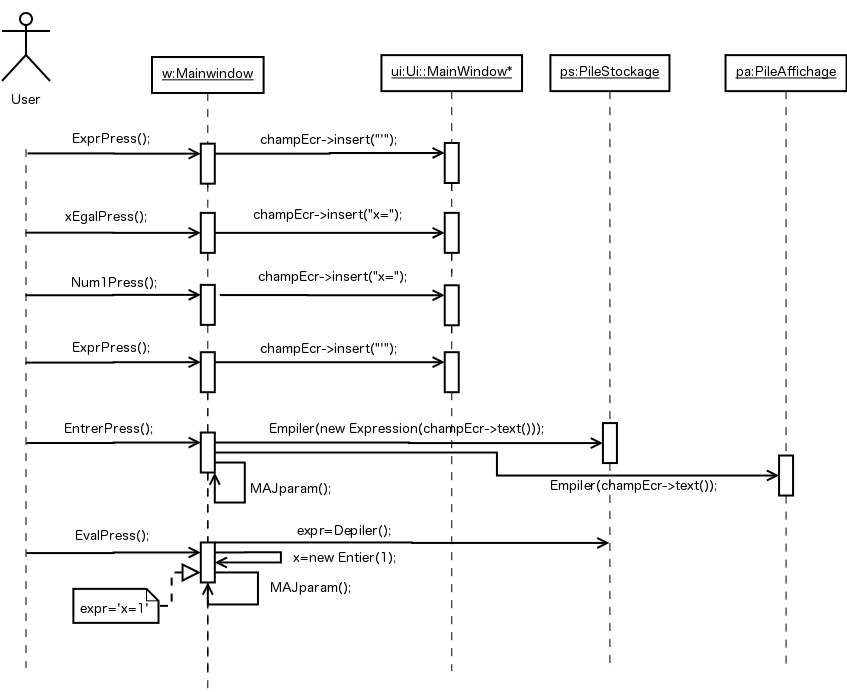
\includegraphics[width=16.7cm]{diag_seq_2.png}
	\caption{Diagramme de s�quence d�crivant le lancement de la fen�tre, la saisie de 'x=1', puis l'�valuation de l'expression et la sauvegarde de la valeur 1 dans la variable x.}
\end{figure}

\section{Impl�mentation}
aaaaaaaah
\end{document}
